\documentclass[13pt,a4paper]{article}

\usepackage[utf8]{inputenc}
\usepackage[russian]{babel}
\usepackage[OT1]{fontenc}
\usepackage{amsmath}
\usepackage{amsfonts}
\usepackage{amssymb}
\usepackage{graphicx}

\usepackage{mathtext}

\usepackage{tikz}
\usepackage{pgfplots}
\usepackage[export]{adjustbox}

\usepackage[left=2cm,right=2cm,top=2cm,bottom=2cm]{geometry}
\usepackage{calc}
\usepackage{wrapfig}
\usepackage{setspace}
\usepackage{indentfirst}
\usepackage{subfigure}


\title{
1.4.1.

Изучение физического маятника
}

\author{Семёнов Андрей Б02-016}
\date{11 марта 2021г.}
\begin{document}

\maketitle
\newpage

\textbf{Цель работы:} исследовать зависимость периода колебаний физического маятника от его момента инерции.


\textbf{В работе используются:} физический маятник (однородный стальной стержень), опорная призма, математический маятник, счетчик числа колебаний, линейка, секундомер.

\section{Теоретические сведения}
Физическим маятником называют любое твердое тело, которое под действием силы тяжести может свободно качаться вокруг неподвижной горизонтальной оси. Движение маятника описывается уравнением:

\begin{equation}
	I\frac{d^2\varphi}{dt^2}=M,
	\label{eq:force_moment}
\end{equation}
где $I$$-$момент инерции маятника, $\varphi$$-$угол отклонения маятника от положения равновесия, $t$$-$время, $M$$-$момент сил, действующих на маятник.\\
\begin{wrapfigure}{r}{0.5\textwidth}
   		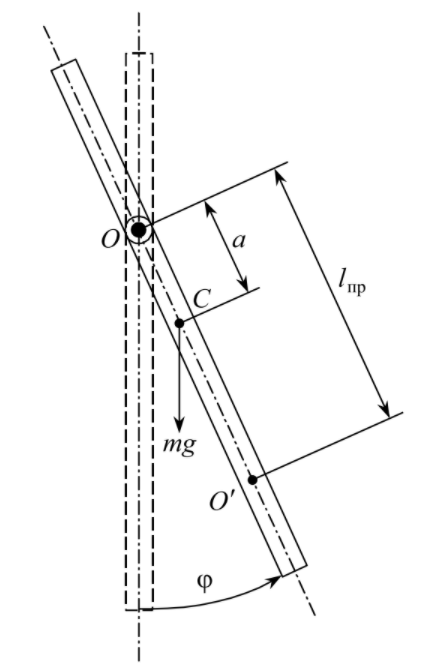
\includegraphics[width=0.4\textwidth]{physpend}
    	\caption{Физический маятник}
    	\label{ris:physpend}
\end{wrapfigure}
В нашей работе в качестве физического маятника \ref{ris:physpend} используется однородный стальной стержень длинны $l$. На стержне закрепляется опорная призма, острое ребро которой является осью качания маятника. Призму можно перемещать вдоль стержня, меняя таким образом расстояние OC от точки опоры маятника до его центра масс. Пусть это расстояние равно $a$, тогда по теореме Гюйгенса-Штейнера:
\begin{equation}
	I=\frac{ml^2}{12}+ma^2,
	\label{eq:inertia_moment}
\end{equation}
Момент силы тяжести равен $M=-mga\sin\varphi$, учтя малость угла $\varphi$ и подставляя это вместе с (\ref{eq:inertia_moment}) в (\ref{eq:force_moment}) получим:
\begin{equation}
	\varphi''+\omega^2\varphi=0,
	\label{eq:osc}
\end{equation}
где 
\begin{equation}
	\omega^2=\frac{ga}{a^2+\frac{l^2}{12}}.
	\label{eq:osc_omega}
\end{equation}
Решением этого уравнение является
\begin{equation}
	\varphi(t)=A\sin(\omega t+\alpha).
	\label{eq:osc_main}
\end{equation}
Амплитуда $A$ и начальная фаза $\alpha$ определяются только только начальными условиями.\\
Период колебаний равен:
\begin{equation}
	T=\frac{2\pi}{\omega}=2\pi\sqrt{\frac{a^2+\frac{l^2}{12}}{ag}}.
	\label{eq:phys_period}
\end{equation}
Видим, что период малых колебаний не зависит ни от фазы, ни от амплитуды колебаний. Изохронность справедлива для всех колебаний, подчиняющихся уравнению (\ref{eq:osc}).\\
Период колебаний математического маятника определяется:
\begin{equation}
	T'=2\pi\sqrt{\frac{l'}{g}}.
	\label{eq:math_period}
\end{equation}
$l'$$-$длина математического маятника. Поэтому величину $l_{pr}=a+\frac{l^2}{12a}$ называют приведённой длиной физического маятника. Точка $O'$ называется центром качания. При качании маятника относительно точки $O'$ егопериод будет таким же, как и при качании относительно точки $O$.  
\begin{wrapfigure}{r}{0.5\textwidth}
   		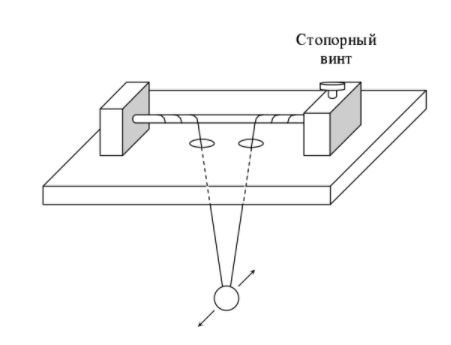
\includegraphics[width=0.4\textwidth]{mathpend}
    	\caption{Математический маятник}
    	\label{ris:mathpend}
\end{wrapfigure}
\newpage
Эти методом можно проверять теоретические сведения. Ещё один метод заключается в проверке правильности формулы (\ref{eq:phys_period}). Входящую в формулу величину $a$ можно изменять, передвигая опорную призму по стержню. В данной работе в качестве математического маятника используется свинцовый шарик, подвешенный на двух расходящихся нитях, как показано на \ref{ris:mathpend}. Длину нитей можно изменять, наматывая их на ось.
\newpage


\section{Выполнение работы}


\subsection{Диапазон амплитуд}


\subsection{Зависимость $T(a)$}


\subsection{График $T^2(a)$}


\subsection{График $T^2(a^2)$}


\subsection{Находим $g/4\pi^2$ и $l^2/12$}


\subsection{Немного математического маятника}
Подберём длину математического маятника так, чтобы в пределах точности измерений периоды колебаний обоих маятников совпали.

\subsection{Обратимость точки подвеса(опоры) и центра качания физического маятника}


\section{Выводы}


\section{Контрольные вопросы}

\textbf{1. При каких упрощающих предположениях была выведена формула (\ref{eq:phys_period})?}\\
\textbf{2. При каком расстоянии от центра масс до точки подвеса период колебаний маятника минимален?}\\
\textbf{3. Как будет вести себя физический маятник, если совместить точку его подвеса с центром масс?}\\
\textbf{4. С какой целью в данной работе математический маятник подвешивается на двух нитях?}\\
\textbf{5. Сформулируйте и докажите теорему Гюйгенса-Штейнера.}
\end{document} 